After performing the task scheduling experiments using \estee{}, our next goal
was to find out how do other aspects of task runtimes (other than the scheduler) affect makespans
of task graph executions, and also to validate some of the rather surprising results of our
experiments, for example the competitiveness of the random scheduler, in a non-simulated setting.
To do that, we had to move from a simulator to a task runtime that can execute task graphs on an
actual distributed cluster.

%TODO: Expand why Dask

We have decided to use \dask{}~\cite{dask} for our experiments,
for several reasons:
\begin{itemize}
	\setlength\itemsep{0.1em}
	\item It is very popular within the scientific community~\cite{dask-user-survey}, therefore any
	      insights on how it could be improved could benefit a wide range of users.
	\item It is implemented in Python, which makes it relatively easy to modify.
	\item It is quite versatile, because it allows executing arbitrary task graphs with dependencies and data
	      objects, and completely supports the task programming model described in \Autoref{ch:taskgraphs}.
	\item It uses a fairly standard distributed architecture with a centralized server that creates task
	      schedules and assigns tasks to a set of distributed workers. This maps well to the cluster
	      architecture used by \estee{}, and also to \gls{hpc} clusters in
	      general.
\end{itemize}

In terms of task scheduling, \dask{} uses a work-stealing scheduler, which has
been tuned extensively to support various use-cases and task graphs. Yet it is unclear whether
additional effort should be directed into improving the scheduler, or if there is another
bottleneck which should be prioritized.

To answer that question, we have analyzed the runtime performance and the bottlenecks of
\dask{} in
\emph{Runtime vs Scheduler: Analyzing Dask's Overheads}\footnote{Note that this line of research follows after the task scheduler analysis described previously
in~\Autoref{ch:estee}, even though it was published at an earlier date.}~\cite{rsds}. This work
provides the following contributions:
\begin{enumerate}
	\item We have created a set of benchmarks containing diverse task graphs implemented in
	      \dask{}. This benchmark set was then used to analyze \dask{}'s
	      performance in various \gls{hpc}-inspired scenarios. We have evaluated the
	      per-task-overhead and scalability of \dask{} and compared how different task
	      scheduling algorithms affect its performance.
	\item We demonstrate that even a naïve (completely random) scheduling algorithm can be in many common
	      situations competitive with the sophisticated hand-tuned work-stealing scheduler used in
	      \dask{}.
	\item We provide \rsds{}, an alternative \dask{} server that is
	      backwards-compatible with existing \dask{} programs and provides significant
	      speed-up vs the baseline \dask{} server in many scenarios, despite using a
	      simpler task scheduler implementation.
\end{enumerate}

Various descriptions of task graph benchmarks, \dask{} and
\rsds{} used in this chapter were adapted from our
publication~\cite{rsds}.

\workshare{I have collaborated on this work with Ada Böhm, we have both contributed to it equally. Source code contribution statistics for
\rsds{} can be found on GitHub\footnoteurl{https://github.com/it4innovations/rsds/graphs/contributors}.}

\section{\dask{} task runtime}
\label{sec:rsds-dask}
% TODO: place Dask into SOTA and describe it more, if not already done in the SOTA chapter
\dask{} is a distributed task runtime implemented in Python that can
parallelise and distribute Python programs. It offers various programming interfaces
(\glspl{api}) that mimic the interfaces of popular Python packages. For example,
\emph{Dask DataFrame} copies the \texttt{pandas}\footnoteurl{https://pandas.pydata.org}
interface for table processing and database operations, \emph{Dask Arrays} copies the
\texttt{numpy}\footnoteurl{https://numpy.org} interface for tensor computations and
\emph{Dask ML} copies the \texttt{scikit-learn}\footnoteurl{https://scikit-learn.org}
interface for machine learning. Thanks to this interface compatibility, existing Python programs
leveraging these libraries can often be parallelised with \dask{} by changing
only a handful of lines of code.

This is demonstrated in~\Autoref{lst:dask-array-example} and~\ref{lst:dask-dataframe-example-2}, which show two
small Python programs that leverage the \emph{Dask Arrays} and \emph{Dask DataFrame}
\gls{api} respectively. Notably, the only difference between these programs
(which are leveraging \dask{}, and thus can be parallelised), and a standard
sequential version, is the change of imports from \texttt{numpy} and
\texttt{pandas} to \dask{} Python modules.

\begin{listing}[h]
	\caption{Example of a Python program that leverages the \dask{} Array
	\gls{api}}
	\label{lst:dask-array-example}
	\begin{minted}[fontsize=\small]{python}
# import numpy as np
import dask.array as np

x = np.random.random((10000, 10000))
y = (y * 2 + x.T).mean(axis=1)
	\end{minted}
\end{listing}

\begin{listing}[h]
	\caption{Example of a Python program that leverages the \dask{} DataFrame
	\gls{api}}
	\label{lst:dask-dataframe-example-2}
	\begin{minted}[fontsize=\small]{python}
# import pandas as pd
import dask.dataframe as pd

df = pd.read_csv("data.csv")

df2 = df[df.y > 0]
df3 = df2.groupby("name").x.std()
	\end{minted}
\end{listing}

\subsection*{Computational model}
\dask{} automatically transforms Python code leveraging these
\glspl{api} into a task graph, which is then executed in parallel, possibly on
multiple nodes of a distributed cluster. This enables almost transparent parallelization of
sequentially looking Python code. However, apart from these high-level interfaces, it is also
possible to build a task graph manually, using the \emph{Futures} interface, to define
complex computational workflows.

The core computational abstraction of \dask{} is a \emph{task graph},
which corresponds closely to the definition of task graphs in \Autoref{ch:taskgraphs}. Each
task represents a single invocation of a Python function. The return value of the function forms
its \emph{output} (a data object), and the arguments of the function invocation define the
\emph{inputs} of the task.

One important aspect of the mapping between Python code and task graphs in
\dask{} is the concept of \emph{partitions}. It is a configuration
parameter that essentially controls the granularity of tasks created by \dask{}
out of Python code that uses its \glspl{api}. For example, a single line of Python
code that performs a query over a \texttt{pandas}-like table (also called DataFrame)
will be eventually converted to a set of individual tasks that e.g.\ perform the query on a subset
of the table's rows. The selected number of these tasks (or partitions) is crucial, since it
determines how effectively will the operation be parallelised. Too few (large) tasks can cause
computational resources to be under-utilized, while too many (small) tasks can overwhelm the
\dask{} runtime.

\subsection*{Architecture}
\dask{} supports multiple computational backends that can execute the task
graphs generated from Python code. The default backend is able to execute the task graph in a
parallelised fashion on a local computer, but there is also a distributed backend called
\emph{Dask/distributed}\footnoteurl{https://distributed.dask.org}
(or simply \emph{distributed}), which is able to execute task graphs on
multiple nodes. Since this backend is most relevant for task graph execution on distributed and
\gls{hpc} clusters, our experiments focus solely on this backend, and any further
reference to \dask{} in this text will assume that it uses the
\emph{distributed} backend.

In terms of architecture, \emph{distributed} is composed of three main components: the
\emph{client}, the \emph{server} and the \emph{worker}. A
single server and an arbitrary number of workers deployed together (e.g.\ on a local machine or a
distributed system) form a \dask{} cluster.

The \emph{client} is a user-facing library that offers various
\glspl{api} used to define computations in Python that can be converted into a task
graph. Once the user defines the computation, the client can connect to the
\dask{} cluster (more specifically, to the server), submit the task graph, wait
for it to be computed and then gather the results. The client can build the whole task graph
eagerly on the user's machine and then send it to the server for processing, however this can
consume a lot of memory and network bandwidth if the task graph is large. For certain types of task
graphs, clients are able to send a much smaller, compressed abstract representation of the task
graph, which is only expanded on the server lazily, which can help reduce memory and network
transfer bottlenecks.

The \emph{server} is the central component of the cluster, which communicates with
the workers and clients through a network, usually a \gls{tcpip} connection,
handles client requests, coordinates task execution on workers and manages the whole
\dask{} cluster. Its main duty is to process task graphs submitted by clients,
by assigning individual tasks to workers, in order to parallelise the execution of the submitted
task graph and in turn efficiently utilize the whole cluster. It uses a sophisticated work-stealing
scheduler that uses many heuristics, which have been tuned for many years. Some of them are
described in the \dask{} manual\footnoteurl{https://distributed.dask.org/en/latest/work-stealing.html}.

The scheduler works in the following way: when a task becomes \emph{ready}, i.e.\
all its dependencies are completed, it is immediately assigned to a worker according to a heuristic
that tries to minimize an estimated start time of the task. This estimate is based primarily on any
potential data transfers that would be incurred by moving the data objects of tasks between
workers, and also the current occupancy of workers. When an imbalance occurs, the scheduler tries
to steal tasks from overloaded workers and distribute them to underloaded workers. The scheduler
also assigns priorities to tasks, which are used by workers to decide which tasks should be
computed first.

The \emph{worker} is a process which executes tasks (consisting of serialized Python
functions and their arguments) that are assigned and sent to it by the server. Workers also
communicate directly amongst themselves to exchange task outputs (data objects) that they require
to execute a task. Tasks assigned to a worker are stored in a local queue, tasks are selected from
it based on their priorities. Each worker can be configured to use multiple threads, some of which
handle network (de)serialization and \gls{io} in general, while the rest is
assigned for executing the tasks themselves. However, there is an important caveat that can limit
the parallel execution of tasks within a worker, which is described below.

\subsection*{Bottlenecks}
The primary bottlenecks that limit the efficiency of \dask{} are related to the
programming language used for its implementation. All described components (server, worker and
client), are implemented in Python, which has non-trivial consequences for its performance, because
the Python language is not well suited for implementing high-performance infrastructure. The most
commonly used Python interpreter (CPython\footnoteurl{https://github.com/python/cpython}) does not allow programmers to
make optimal use of hardware in general in an easy way, due to its indirect memory layout and
automatic memory management that pervasively uses reference-counting.

Crucially, there is a specific quirk of this interpreter that can severely reduce the performance
of task graph execution in \dask{}, and specifically affects the
characteristics of its workers. The CPython interpreter infamously uses a shared, per-process lock
called \gls{gil}, which synchronizes access to the interpreter internals. This
means that when a Python program is interpreted using CPython, only a single thread that executes
Python code can make progress at the same time. It is still possible to achieve concurrency with
multiple Python threads (e.g.\ by using blocking \gls{io}, which releases the
\gls{gil} while the thread is blocked), but not parallelism, under this design.
There are some caveats to this, notably code written using native Python extensions (most commonly
written in \texttt{C}, \texttt{C++} or \texttt{Rust})
can run truly in parallel with other Python threads, but only if it opts into releasing the global
lock, and if it does not need to interact with the Python interpreter at all while the native code
is running.

The \gls{gil} issue does not impact only \dask{}, of course.
It is a pervasive issue across the whole Python ecosystem. There have been multiple attempts over
the years to remove the \gls{gil} from CPython, but they have not been successful
yet. The most recent attempt has progressed the furthest, and it has been accepted as a
\gls{pep} 703~\cite{pep703}, so it is possible that the
\gls{gil} will be eventually removed from CPython. However, even if this proposal
is eventually adopted, it will probably take years before Python packages and programs will fully
adapt to the change.

The presence of the \gls{gil} poses a challenge for \dask{}
workers. Unless a task executed by a worker releases the \gls{gil} (which essentially means that the task either has to be
implemented in native code, or it needs to block on an \gls{io} operation), it will block
all other tasks from executing at the same time. Therefore, a single \dask{}
worker can only execute at most one non-native and non-blocking task at once, which can potentially
severely limit its throughput and the efficiency of task graph execution. It is worth noting that
many commonly used data science and data analysis tasks executed with \dask{}
will likely be implemented in native code (such as \emph{numpy},
\emph{pandas}, or their \dask{} equivalents). However, for tasks
written in pure Python, the worker will essentially behave in a singlethreaded fashion. This has
been observed for example in~\cite{dasksparkcomparison}, where several workflows did not benefit
at all from multithreaded \dask{} workers.

To alleviate this limitation, \dask{} workers can be executed in multiple
copies on the same node, each running inside a separate process. In this setup, each worker has its
own copy of the CPython interpreter, and therefore also its own copy of the
\gls{gil}, and thus tasks running inside one worker do not affect (and most
importantly, block) tasks running on other workers. However, this also means that certain overhead
(a \gls{tcpip} connection to the server, a worker entry in the scheduler,
management of worker tasks) is multiplied by the number of spawned workers on each node. In certain
cases, it is thus necessary to carefully balance the trade-off between too few workers (which can
hamper task execution parallelism) and too many workers (which can reduce the overall efficiency of
the \dask{} runtime).

\section{\dask{} runtime overhead analysis}
\label{sec:rsds-dask-overhead-analysis}
We have designed a series of experiments to evaluate the inner overhead of
\dask{} and to find out which factors affects its runtime performance the most.

\subsection*{Benchmarks}
To evaluate the runtime, we have prepared a diverse set of benchmarks that span from simple
map-reduce aggregations to text processing workloads and table queries. The properties of the task
graphs used in our experiments along with the \dask{}
\gls{api} that was used to create them are summarized in
Table~\ref{tab:dask-graph-properties}.

\setlength{\tabcolsep}{5pt}
\begin{table}
	\caption{Properties of \dask{} benchmark task graphs}
	\centering
	\label{tab:dask-graph-properties}
	\begin{tabular}{l|rrrrrc}
		\toprule
		\textbf{Task graph} & \textbf{\#T} & \textbf{\#I}       & \textbf{S} &
		\textbf{AD}         & \textbf{LP}  & \textbf{\gls{api}}                               \\
		\midrule
		merge-10K           & 10001        & 10000              & 0.027      & 0.006 & 1  & F \\
		merge-15K           & 15001        & 15000              & 0.027      & 0.006 & 1  & F \\
		merge-20K           & 20001        & 20000              & 0.027      & 0.006 & 1  & F \\
		merge-25K           & 25001        & 25000              & 0.027      & 0.006 & 1  & F \\
		merge-30K           & 30001        & 30000              & 0.027      & 0.006 & 1  & F \\
		merge-50K           & 50001        & 50000              & 0.027      & 0.006 & 1  & F \\
		merge-100K          & 100001       & 100000             & 0.027      & 0.006 & 1  & F \\
		merge\_slow-5K-0.1  & 5001         & 5000               & 0.023      & 100   & 1  & F \\
		merge\_slow-20K-0.1 & 20001        & 20000              & 0.023      & 100   & 1  & F \\
		tree-15             & 32767        & 32766              & 0.027      & 0.007 & 14 & F \\
		xarray-25           & 552          & 862                & 55.7       & 3.1   & 10 & X \\
		xarray-5            & 9258         & 14976              & 3.3        & 0.4   & 10 & X \\
		bag-25K-10          & 236          & 415                & 292        & 1233  & 6  & B \\
		bag-25K-100         & 21631        & 41430              & 3.2        & 13.9  & 8  & B \\
		bag-25K-200         & 86116        & 165715             & 0.8        & 3.6   & 9  & B \\
		bag-25K-50          & 5458         & 10357              & 12.6       & 54.9  & 7  & B \\
		bag-50K-50          & 5458         & 10357              & 25.2       & 214   & 7  & B \\
		numpy-50K-10        & 209          & 228                & 70108      & 169   & 7  & A \\
		numpy-50K-100       & 19334        & 21783              & 760        & 2.6   & 10 & A \\
		numpy-50K-200       & 77067        & 86966              & 191        & 0.9   & 11 & A \\
		numpy-50K-50        & 4892         & 5491               & 2999       & 8.3   & 9  & A \\
		groupby-2880-1S-16H & 22842        & 31481              & 1005       & 11.9  & 9  & D \\
		groupby-2880-1S-8H  & 45674        & 62953              & 503        & 7.7   & 9  & D \\
		groupby-1440-1S-1H  & 182682       & 251801             & 64.3       & 3.8   & 10 & D \\
		groupby-1440-1S-8H  & 22842        & 31481              & 503        & 7.7   & 9  & D \\
		groupby-360-1S-1H   & 45674        & 62953              & 64.3       & 3.8   & 9  & D \\
		groupby-360-1S-8H   & 5714         & 7873               & 503        & 8.0   & 8  & D \\
		groupby-90-1S-1H    & 11424        & 15743              & 64.3       & 3.9   & 8  & D \\
		groupby-90-1S-8H    & 1434         & 1973               & 501        & 7.7   & 7  & D \\
		join-1-1S-1H        & 673          & 1224               & 15.3       & 33.0  & 5  & D \\
		join-1-1S-1T        & 72001        & 125568             & 3.7        & 1.7   & 11 & D \\
		join-1-2s-1H        & 673          & 1224               & 9.3        & 9.8   & 5  & D \\
		vectorizer-1M-300   & 301          & 0                  & 10226      & 1504  & 0  & F \\
		wordbag-100K-50     & 250          & 200                & 5136       & 301   & 2  & F \\
		\bottomrule
	\end{tabular}\\
	\vspace{1mm}

	\#T = Number of tasks; \#I = Number of dependencies; \\
	S = Average task output size [KiB]; AD = Average task
	duration [ms]; \\ LP = longest oriented path in the graph; \\ D = DataFrame; B
	= Bag; A = Arrays; F = Futures; X = XArray
\end{table}

Most of the task graphs are heavily inspired by programs from the \dask{}
Examples repository\footnoteurl{https://examples.dask.org}. The definitions of the benchmarks are available in
a GitHub repository\footnoteurl{https://github.com/It4innovations/rsds/blob/master/scripts/usecases.py}. A short summary of the individual benchmarks is
provided below.

\noindent\textbf{merge-n} creates $n$ independent trivial tasks
that are merged at the end (all of their outputs are used as an input for a final merge task). This
benchmark is designed to stress the scheduler and the server, because the individual tasks are very
short (essentially they do no work).

\noindent\textbf{merge\_slow-n-t} is similar to \texttt{merge-n}, but with longer,
$t$ second tasks.

\noindent\textbf{tree-n} performs a tree reduction of $2^n$
numbers using a binary tree with height $n-1$.

\noindent\textbf{xarray-n} calculates aggregations (mean, sum) on a
three-dimensional grid of air temperatures~\cite{airdataset}, $n$
specifies size of grid partitions.

\noindent\textbf{bag-n-p} works with a dataset of $n$ records in
$p$ partitions. It performs a cartesian product, filtering and aggregations.

\noindent\textbf{numpy-n-p} transposes and aggregates a two-dimensional
distributed NumPy array using the \emph{Arrays} interface. The array has size
$(n,n)$ and it is split into partitions of size $(n/p,n/p)$.

\noindent\textbf{groupby-d-f-p} works with a table with $d$ days of
records, each record is $f$ time units apart, records are partitioned by
$p$ time units. It performs a groupby operation with an aggregation.

\noindent\textbf{join-d-f-p} uses the same table, but performs a self-join.

\noindent\textbf{vectorizer-n-p} uses
Wordbatch\footnoteurl{https://github.com/anttttti/Wordbatch}, a text processing library, to compute hashed features of
$n$ reviews from a TripAdvisor dataset~\cite{wordbatcharticle} split
into $p$ partitions.

\noindent\textbf{wordbag-n-p} uses the same dataset, but computes a full text processing
pipeline with text normalization, spelling correction, word counting and feature extraction.

\subsection*{Benchmark configuration}
Our experiments were performed on the Salomon supercomputer\footnoteurl{https://docs.it4i.cz/salomon/introduction}. Each
Salomon node has two sockets containing Intel Xeon E5-2680v3 with 12 cores clocked at
$2.5$ GHz ($24$ cores in total),
$128$ GiB of \gls{ram} clocked at $2133$
MHz and no local disk. The interconnections between nodes use a InfiniBand FDR56 network with 7D
enhanced hypercube topology.

Unless otherwise specified, by default we spawn $24$
\dask{} workers per node, each using a single thread for task computations. We
chose this setting because of the CPython \gls{gil} issue described earlier.
Since our benchmarks are mostly compute-bound and not \gls{io}-bound, a single
worker cannot effectively use more than a single thread. Not even the popular
\texttt{NumPy} and \texttt{Pandas} libraries used in our benchmarks are
multithreaded by default, which is also why \dask{} provides direct
\gls{api} support for their parallelization. Using the same number of workers as
the available cores ensures that no more than a single task per core is executed at any given
moment, to avoid oversubscription of the cores.

To validate our choice of this default configuration, we have benchmarked a configuration using a
single worker with $24$ threads per each node. We have found that it provides
no benefit in comparison to a single worker with only one thread in any of our benchmarks.

For each of our experiments, we state the number of used worker nodes, which contain only the
workers. We always use one additional node which runs both the client and the server. For our
scaling experiments, we use $1$ to $63$ worker nodes
($24$-$1512$ \dask{} workers), for
the rest of our experiments we use either $1$ or $7$
worker nodes ($24$ or $168$ \dask{}
workers). We have chosen these two cluster sizes to represent a small and a medium sized
\dask{} cluster. The number of workers is fixed, they do not connect nor
disconnect during the computation. The timeout for all benchmarks was set to
$300$ seconds.

We have executed each benchmark configuration five times (except for the scaling benchmarks, which
were executed two times to lower our computational budget) and averaged the result. We have
measured the duration (\emph{makespan}) between the initial task graph submission to
the server and the processing of the final output task by the client. The whole cluster was reset
between each benchmark execution.

The following abbreviations are used in figures with benchmark results: \emph{ws}
marks the work-stealing scheduler and \emph{random} represents the random scheduler.

\subsection*{Evaluation}
We have designed three specific experiments, which focus on \dask{}'s
scheduler, on its inner overhead, and on the effect of \gls{gil} on its
performance.

\subsubsection*{Random scheduler}
Our original goal of this experiment was to test how different schedulers affect the performance
characteristics of \dask{}. However, it turned out that plugging a different
scheduling algorithm into it is quite complicated, because it uses a work-stealing scheduler
implementation that is firmly ingrained into its codebase across multiple places. There was not a
single place where the scheduler could be swapped for a different implementation without affecting
other parts of the runtime (like it is possible in \estee{}). Integrating a
different complex scheduler into \dask{} would thus require making further
changes to it, which could introduce bias stemming from arbitrary implementation decisions.

We have thus decided to implement perhaps one of the simplest schedulers possible, which does not
require complex state and which could be implemented relatively easily within
\dask{} -- a fully random scheduler. This scheduler simply uses a
\gls{prng} engine to assign tasks to workers at random. Our
\estee{} experiments have shown that a completely random scheduler could still
achieve competitive performance in some cases, which was a quite surprising result to us. However,
since these results were only tested in a simulated setting, it was interesting to examine how it
would fare on an actual distributed cluster, scheduling real-world \dask{} task
graphs.

\begin{figure}
	\centering
	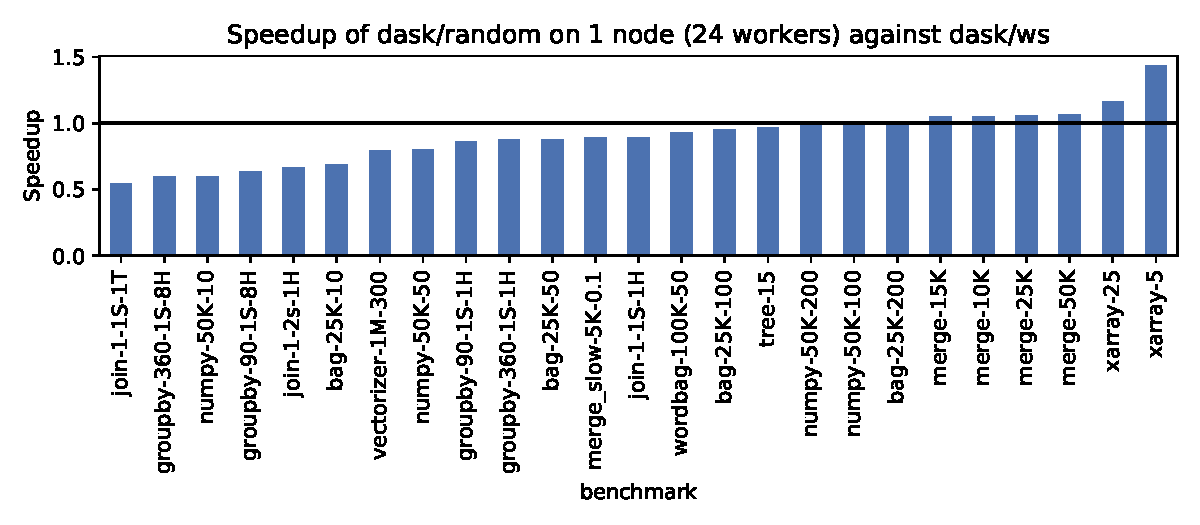
\includegraphics[width=0.9\textwidth]{imgs/rsds/charts/speedup-dask-random-1}
	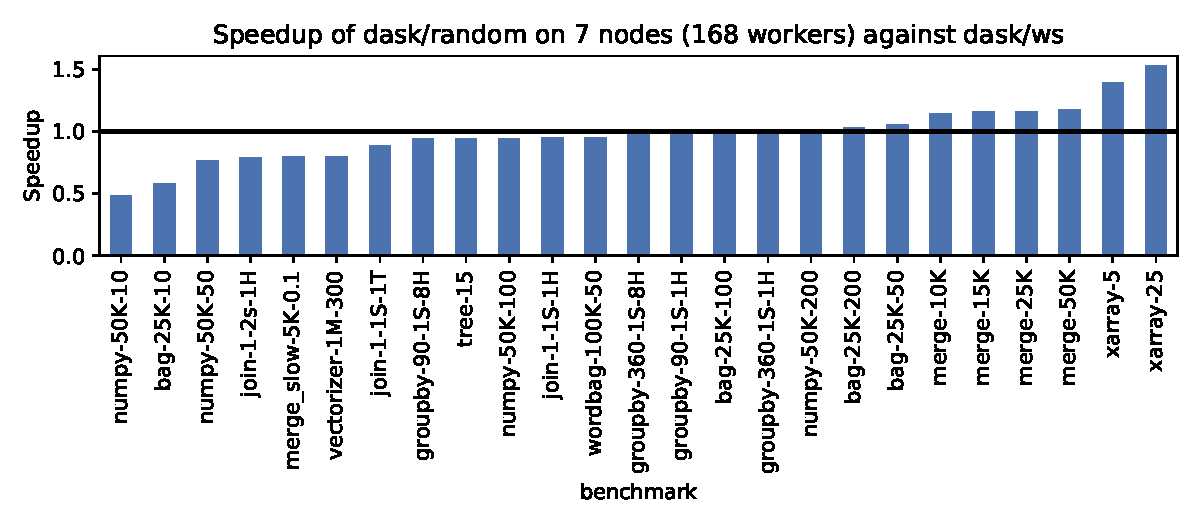
\includegraphics[width=0.9\textwidth]{imgs/rsds/charts/speedup-dask-random-7}
	\caption{Speedup of \dask{}/random scheduler; \dask{}/ws is baseline.}
	\label{fig:dask-ws-vs-random}
\end{figure}

We can observe the results of benchmarks that compare \dask{} using its
baseline work-stealing scheduler vs a completely random scheduler in \Autoref{fig:dask-ws-vs-random}.
Based on these results, it is clear that the random scheduler fares relatively well on both small
and medium sized clusters. At worst, it produces a twice longer makespan, but overall it is quite
close to the performance of the work-stealing scheduler, and in some cases it even outperforms it
with a $1.4\times$ speedup.

If we aggregate the results with a geometric mean, the random scheduler achieves
$88\%$ of the performance of the work-stealing scheduler with a single node,
and $95\%$ with seven nodes. The performance of the random scheduler thus gets
closer to the performance of work-stealing when more workers are used.

The fact that the random scheduler's performance improves with a larger number of nodes is not
surprising. With more nodes, it is easier to fully saturate the potential parallelism contained in
each task graph. Furthermore, a random scheduler produces less network traffic, and has much
smaller computational cost on the server; as we will see in the next experiment, the work-stealing
scheduler's computational cost increases notably when more workers are present.

Furthermore, for certain task graphs, a complex scheduling algorithm might not be needed, and a
random schedule is sufficient to achieve reasonable results. However, all of that combined is still
a rather weak explanation for why is a random scheduler so competitive with the work-stealing
scheduler in \dask{}. In the following experiments, we will show that
\dask{} has considerable runtime overhead, which might introduce a bottleneck
that is more impactful than the effect of the used schedule. In the next section
(\ref{sec:rsds-description}), we will see that with a more efficient runtime and less server
overhead, random schedules will become less competitive.

%There are two effects that explain the reasonable performance of the random scheduler. Firstly, the
%computational complexity of work-stealing scales with the number of available workers. With more
%workers, the work-stealing scheduler has to perform more work to compute where should the tasks be
%computed, and it also generates additional network traffic by sending task stealing messages
%between workers. On the other hand, a random scheduler has a fixed computation cost per task,
%completely independent of the worker count, as it simply chooses a worker randomly, and it also
%sends no additional network messages other than one worker assignment per task. The difference in
%computational overhead between these two schedulers will be examined in more detail in the
%following experiment.

%The second effect is also related to the fact that the random scheduler performs better with more
%workers. Our benchmark set is compute-bound, so if there is a large enough number of workers
%(relative to the number of tasks), it might not be that difficult for the scheduler to saturate all
%the workers, even with a random schedule, as long as the task graph structure is not very
%complicated. Furthermore, if the scheduler wants to utilize all computational power of a cluster
%with many workers, network transfers are less avoidable, which decreases the chance that a random
%scheduler induces an unnecessary data transfer that could have been avoided by a smarter scheduler.

%The results of this experiment suggest that in certain scenarios, a complex scheduling algorithm is
%not needed and a random schedule is sufficient for \dask{}. This shows that the
%scheduler might not be its main bottleneck. We will also examine this in the following experiments.

\subsubsection*{Overhead per task}
\label{sec:dask-overhead-per-task}
We have seen that a random scheduler can be surprisingly competitive with the work-stealing
scheduling implementation in \dask{}. In this experiment, we further examine
this effect by estimating the inner overhead of \dask{} per each executed task.
In order to isolate the effects of the specific executed tasks, and network communication and
worker overhead, we have implemented a special implementation of the \dask{}
worker that we label \emph{zero worker}.

Zero worker is a minimal implementation of the \dask{} worker process, written
in Rust. Its purpose is to simulate a worker with infinite computational speed, infinitely fast
worker-to-worker transfers and zero additional overhead. It actually does not perform any real
computation; when a task is assigned to a zero worker, it immediately returns a message that the
task was finished. It also remembers a set of data-objects that would be placed on the worker in a
normal computation. When a task requires a data object which is not in this list, the worker
immediately sends a message to the server, claiming that the data object was placed on it -- this
simulates an infinitely fast download of data between workers. No actual worker-to-worker
communication is performed in such case.

Zero workers respond to every data object fetch request with a small mocked constant data object.
Such requests come from the server when a client asks for a data object, usually at the end of the
computation. Since there is no worker-to-worker communication when the zero worker is used, fetch
requests never come from other workers.

This idealized worker implementation helps us to understand the fundamental overhead of the
\dask{} runtime, independent of the specific tasks that are being executed.
Note that even though all tasks in this mode are basically the same, the shape and size of the
benchmarked task graph are still important, since they affect the scheduler's performance and also
bookkeeping overhead of the runtime.

\begin{figure}
	\centering
	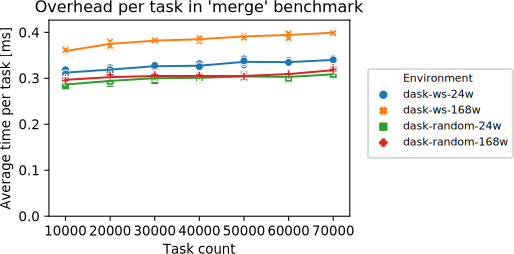
\includegraphics[width=0.5\textwidth]{imgs/rsds/charts/dask-merge-task-scaling}
	\caption{Overhead per task in \dask{} with an increasing number of tasks.}
	\label{fig:dask-merge-task-scaling}
\end{figure}

Using this special mode, we have evaluated the average runtime overhead per each task, which is
calculated as the total makespan divided by the number of tasks in the executed task graph.
\Autoref{fig:dask-merge-task-scaling} shows the average overhead per task for the \texttt{merge}
benchmark, we can see the average overhead per each task (the Y axis), and how it changes with an
increasing number of tasks (X axis). We can observe that the overhead of the random scheduler is
smaller the overhead of the work-stealing scheduler, as expected. We can also see that the overhead
per task increases with an increasing number of tasks, for both schedulers. There is also a
distinct increase of overhead between the overhead with $24$ workers (one
node) and $168$ workers (seven nodes) for the work-stealing scheduler.

\begin{figure}
	\centering
	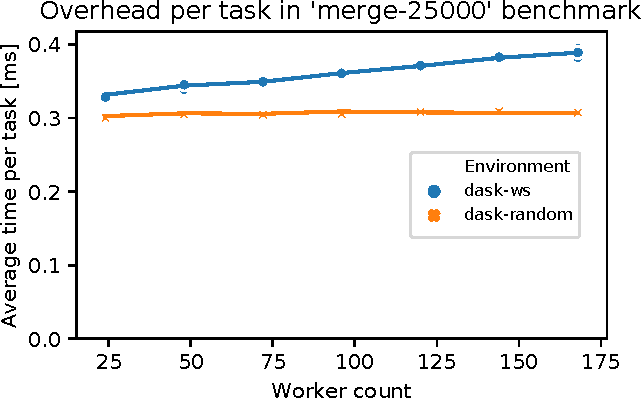
\includegraphics[width=0.5\textwidth]{imgs/rsds/charts/dask-merge-worker-scaling}
	\caption{Overhead per task in \dask{} with an increasing number of workers.}
	\label{fig:dask-merge-worker-scaling}
\end{figure}

This can be examined in more detail in \Autoref{fig:dask-merge-worker-scaling}, which shows how does the
overhead increase when more workers are available. It is clear that the performance of the
work-stealing degrades rapidly when more workers are added to the custer, while the overhead of th
random scheduler stays almost constant, inependent on the number of workers.

The \dask{} manual states that ``Each task suffers about 1ms of overhead. A
small computation and a network roundtrip can complete in less than
10ms.''~\footnote{\url{https://distributed.dask.org/en/latest}}. Our experiment shows that the overhead is less than
$1ms$ for most of our benchmarks.

\begin{figure}
	\centering
	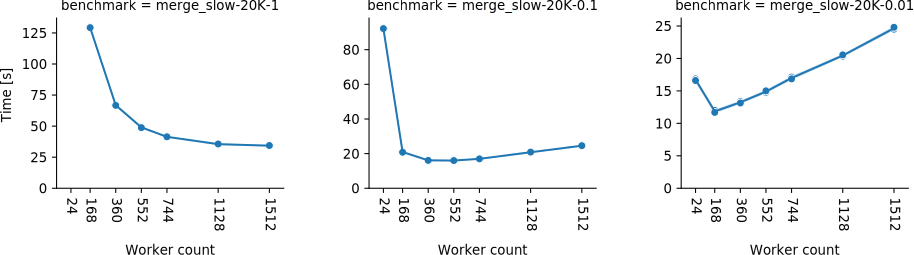
\includegraphics[width=0.9\textwidth]{imgs/rsds/charts/dask-strong-scaling}
	\caption{Strong scaling of \dask{} with different task durations
	($1000ms$, $100ms$ and
	$10ms$).}
	\label{fig:dask-strong-scaling}
\end{figure}

The overhead per task is an important property of the task runtime, since it determines the minimal
duration of a task that is still viable for parallel execution with that runtime. If the duration
of a task is similar or smaller than the overhead of the runtime itself, executing such task with
the runtime will probably not yield any speedup. This is demonstrated in
\Autoref{fig:dask-strong-scaling}, which shows the strong scaling of \dask{} on the
$merge\_slow$ benchmark. The three charts demonstrate its scaling with tasks that take
$1000ms$, $100ms$ and $10ms$ respectively.
With tasks that take a second, \dask{} is able to scale relatively well up to
$1512$ workers. However, when tasks take ten times less time, it only scales up
to around $360$ workers, and when tasks take only $10ms$,
\dask{} scales to around $168$ workers, and adding further
workers makes the makespan longer.

The results of this experiment indicate that the general runtime overhead of
\dask{} mainly grows with an increasing number of tasks, no matter which
scheduler is used. On the other hand, overhead of the work-stealing scheduler grows primarily with
the number of workers. They also show that the minimum duration of tasks executed by
\dask{} should be taken into account, to avoid introducing too much runtime
overhead.

These results also suggest that \dask{} can struggle with a larger number of
workers. This would not be an issue on its own, as every task runtime will have its scaling limit.
However, due to the already mentioned effect of \gls{gil},
\dask{} users might be forced to use more workers than would be otherwise
necessary to achieve reasonable performance. We will examine this in the next experiment.

\subsubsection*{The effect of \gls{gil}}
As noted earlied, the \gls{gil} can have a non-trivial effect on the performance
of Python programs. This can also be seen in \dask{}, where the configuration
of workers might need to be tuned in order to achieve optimal performance.

\begin{figure}
	\centering
	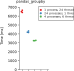
\includegraphics[width=0.3\linewidth]{./imgs/rsds/charts/dask-gil-scaling}
	\caption{Effect of \gls{gil} on the performance of the \emph{pandas\_groupby} benchmark}
	\label{fig:dask-gil-scaling}
\end{figure}

\Autoref{fig:dask-gil-scaling} demonstrates the effect of \gls{gil} on the
\emph{pandas\_groupby} benchmark. We have executed the same benchmark using three
\dask{} worker configurations on a single node. In the default configuration,
with a single worker that uses $24$ threads (one for each core), the pipeline
finishes in approximately $6.5$ seconds. If we instead create a single worker
per each core ($24$ processes, each with a single thread), the performance
improves significantly, by $35\%$! This makes it clear that the
\gls{gil} is a bottleneck in this case, and more \dask{}
workers are needed to improve performance by enabling parallel task execution.

However, it is not so simple as to always use a single \dask{} worker per core.
As we have discovered with our earlier benchmarks, more workers introduce non-negligible overhead
for the \dask{} server. This can be seen from the result of the third
configuration, which uses $4$ \dask{} workers
(processes), each leveraging $6$ threads. This configuration actually
achieves the best performance out of the three tested configurations. It is thus clear that for
some \dask{} workflows, users might need to carefully tune the configuration of
workers to achieve optimal performance.

\subsubsection*{Summary}
Our experiments have shown that \dask{} does not scale optimally to a large
number of workers and it might require manual tuning of worker configuration to achieve the optimal
performance. This lead us to the idea of improving the implementation of the
\dask{} server, in order to reduce its overhead in \gls{hpc}
scenarios.

\section{\rsds{} task runtime}
\label{sec:rsds-description}
In order to examine how much could the performance of \dask{} be improved if we
were able to reduce its runtime overhead, we have developed \rsds{} (Rust \dask{} server), an
open-source drop-in replacement for the \dask{}
server\footnoteurl{https://github.com/it4innovations/rsds}, with the following goals:

\begin{itemize}
	\item Keep backwards compatibility with existing \dask{} programs, so that it can be
	      used to speed up existing workflows. This also enables us to compare the performance of
	      \rsds{} and \dask{} on the benchmarks described in the
	      previous section.
	\item Design an efficient runtime that could scale to \gls{hpc} use-cases, to find a
	      baseline for how much fast could \dask{} become if its overhead was reduced.
	\item Use a modular architecture that would enable easily replacing the implementation of the scheduler,
	      to enable easier experimentation with scheduling algorithms on non-simulated distributed clusters.
\end{itemize}

\subsection*{Architecture}
\rsds{} is implemented in the Rust programming language, which has a minimal
runtime and does not dictate automatic memory management. This reduces the ubiquitous overhead of
reference counting and data indirection present in Python. It also has direct support for
asynchronous \gls{io} and provides strong memory safety guarantees, hence it is
well suited for writing distributed applications.

\begin{figure}[h]
	\centering
	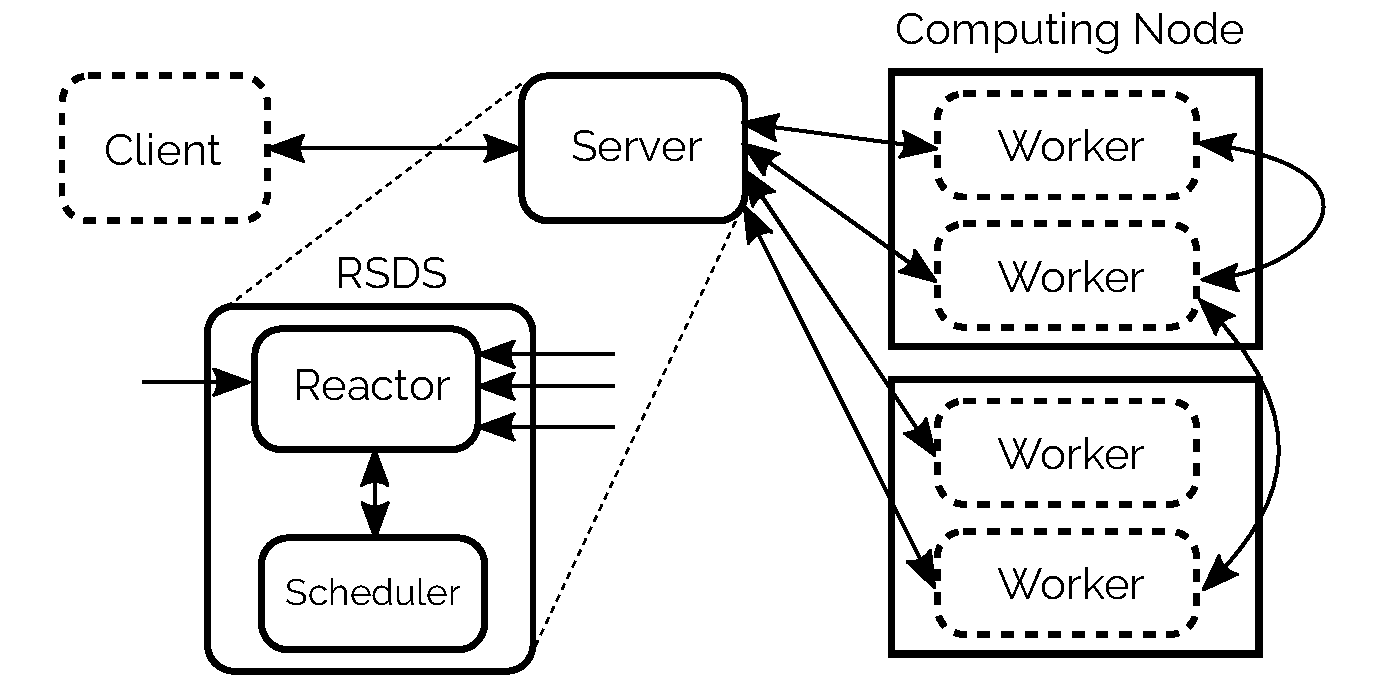
\includegraphics[width=0.8\linewidth]{./imgs/rsds/rsds-architecture}
	\caption{Architecture of \rsds{} (\dask{} components are dashed)}
	\label{fig:rsds-architecture}
\end{figure}

The architecture of \rsds{} is shown in \Autoref{fig:rsds-architecture}. It reuses
the client and worker components from \dask{}, but replaces its server (and
therefore also the scheduler). The main architectural difference between the two implementations is
that \rsds{} separates the server into two parts: \emph{reactor}
and \emph{scheduler}. The reactor manages worker and client connections, maintains
bookkeeping information and translates scheduler assignments into \dask{}
network messages which are then sent to the workers.

The scheduler is a process which receives a task graph and outputs assignments of tasks to workers.
It does not know about network connections, the \dask{} network messages or any
other bookkeeping that is not relevant to scheduling. Since it is isolated, it can be easily
swapped, and therefore it is trivial to experiment with different schedulers in
\rsds{}. Another benefit is that we can easily run the scheduler in a separate
thread to enable concurrent scheduling and runtime management. This is possible because the
scheduler does not share any data structures with the reactor. A disadvantage of this scheme is
that the both the reactor and the scheduler need to build their own task graph, which increases
memory usage, but we have not found this to be a problem in practice.

\subsection*{Compatibility with \dask{}}
The individual \dask{} components communicate together using a custom
communication protocol that contains dozens of different message types. Messages are represented as
dictionaries, where a single field specifies the type of the message and the rest of the fields
contain parameters specific to the given message type.

\dask{} splits messages into multiple parts called \emph{frames}
and serializes each frame with the MessagePack\footnoteurl{https://msgpack.org} binary serialization
format. The messages are split mostly for performance reasons. If a client sends large binary data
to a worker (or vice-versa), the server can deserialize only the first frame containing the message
metadata, and it does not need to further process the binary data, it merely forwards it to the
correct destination. The protocol is designed in such a way that any Python specific objects sent
within the protocol are fully opaque to the server. For example, the server does not need to
understand Python function definitions, it only forwards them from clients to workers, where they
are deserialized and executed. This makes it possible to implement the central server in a
different language than Python.

To retain compatibility with existing \dask{} programs,
\rsds{} must understand this protocol, and be able to both read and also
generate its messages. However, reimplementing the protocol was relatively challenging, because of
two reasons. The first reason is that the protocol is unfortunately mostly
undocumented\footnoteurl{https://github.com/dask/distributed/issues/3357}, and its exact definition depends solely on
\dask{} code that creates the protocol messages ad-hoc in many different source
files and locations. We thus had to reverse-engineer its functionality based on the original
\dask{} source code.

The second reason is that \dask{} makes heavy use of the fact that Python is a
very flexible and dynamic language in its frame encoding scheme. The specific rules of this
encoding grew organically over time and they have become quite complicated and dynamic, as
\dask{} can split messages into frames almost arbitrary ways. Specifically, it
sometimes extracts values out of arbitrary array indices or dictionary keys into a separate frame
during serialization, and then puts them back into the original place during deserialization. The
encoded frame metadata then contains a series of array index and dictionary key accessors. For
example, \verb|[0, "attr1", 1]: <data>| tells the deserializer to put the specified data into the
second element of an array located in the \texttt{"attr1"} key of a dictionary that is
located at the first element of the input array contained within the frame. This dynamic frame
(de)fragmentation is relatively straightforward to perform in a dynamic language like Python, but
it becomes incredibly difficult to handle in a statically-typed language with a strict type system,
such as Rust.

A related issue is that \dask{} sometimes uses a completely different frame
encoding scheme, even for the same message type, which further complicates frame deserialization.
In order to overcome these challenges, we made a small change to the \dask{}
protocol, to make it feasible to implement the server in a statically typed language, which does
not make it trivial to parse the flexible messages generated by \dask{} clients
and workers.

\begin{figure}
	\centering
	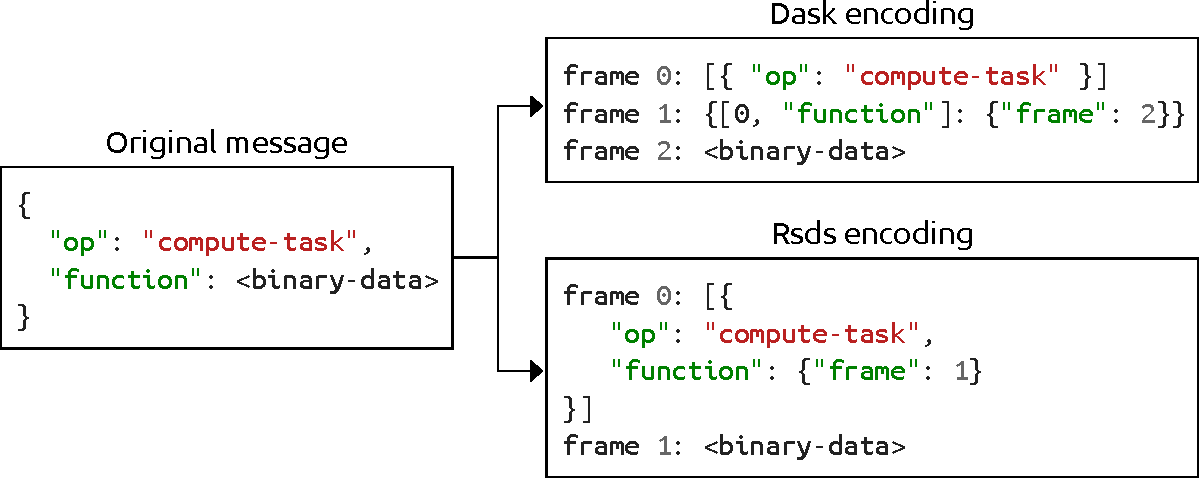
\includegraphics[width=0.9\columnwidth]{./imgs/rsds/frame-encoding}
	\caption{\dask{} message encoding}
	\label{fig:rsds-dask-frame-encoding}
\end{figure}

Our modification changes the dynamic encoding of \dask{} messages into frames.
We have modified it in a way that always keeps the original message structure, so that it is easier
to deserialize. This modification is described in \Autoref{fig:rsds-dask-frame-encoding}, which contains a
simplified scheme that depicts a \dask{} message, and its encoding in
\dask{} and in \rsds{}\footnote{Note that the message and the encoding is depicted using a \gls{json}
notation, for improved readability. In reality, the data is encoded using MsgPack.}. On the
left, we can see the message (dictionary) that we want to serialize, which contains two fields
(\texttt{op} and \texttt{function}). The original
\dask{} encoding, shown in the top right corner, would fragment this dictionary
by removing its \texttt{function} field and moving it to a separate frame. During
deserialization, the field would have to be put back into the original message, transmitted in the
first frame. Our modified encoding, shown in the bottom right corner, instead keeps the original
message structure, but replaces the field that has to be transferred in a separate frame with a
placeholder. During deserialization, the placeholder is replaced with the contents of the second
frame, which is relatively easy to implement in a statically typed language, because it avoids the
need to dynamically change the message structure during deserialization.

This protocol change only modifies low-level message handling, and it is thus fully transparent to
the rest of the code, and spans less than 100 modified lines of \dask{} source
code. Crucially, it has no effect on the functionality of clients, workers and the server, so it
does not require any modifications in \dask{} user programs. Our modified
version of \dask{} is open-source and available
online\footnoteurl{https://github.com/kobzol/distributed/tree/simplified-encoding}. Note that all evaluations presented in this chapter use the
modification described above. We have benchmarked this modification and found that there are no
performance differences in respect to the original \dask{} message encoding.

\rsds{} does not actually implement all \dask{} message
types. Some of them are rarely used, and their implementation would be highly complex, for minimal
gain, and some of them cannot be implemented in a straightforward way in a different language than
Python. For example, Dask contains an \gls{api} that allows clients to run a
Python function on the server, yet this functionality does not have a direct counterpart in a
server implemented in a different programming language. The fact that \rsds{}
is able to execute all the benchmarks described in~\Autoref{sec:rsds-dask-overhead-analysis} demonstrates that it
supports a wide variety of \dask{} programs.

\subsection*{Schedulers}
We have implemented two schedulers in \rsds{}, to allow us comparing its
performance to \dask{} -- a work-stealing scheduler and a completely random
scheduler.

Even though it was not possible to exactly replicate the work-stealing implementation used in
\dask{}, since it is affected by a very large amount of implementation choices
and details, our implementation is inspired by it. However, it is also deliberately kept simple, to
avoid the need to perform extensive hand-tuning of constants and parameters within the scheduler.
Some of the heuristics used by \dask{} were changed, simplified, or dropped in
our implementation. For example \rsds{}, does not estimate average task
durations and does not use any network bandwidth estimates.

The \rsds{} work-stealing scheduler works as follows: when a task becomes ready
(i.e.\ all its inputs are already finished), it is immediately assigned to a worker. The scheduler
chooses a worker where the task may be executed with minimal data transfer costs, while it
deliberately ignores the load of the worker. The load is ignored to speed up the decision in
optimistic situations when there is enough tasks to keep the workers busy. When it is not the case,
it is solved by balancing, which is described below.

When a new task is scheduled or when a task is finished, the scheduler checks if there are nodes
that are under-loaded. In such case, balancing is performed and the scheduler reschedules tasks
from workers with a sufficient number of tasks to under-loaded workers. During rescheduling, the
scheduler simply passes the new scheduling state to the reactor, which performs all of the complex
rescheduling logic. It tries to retract rescheduled tasks from their originally assigned workers.
If retraction succeeds, the task is scheduled to the newly assigned worker. When the retraction
fails, because a task is already running or it has been finished, the scheduler is notified and it
then initiates balancing again, if necessary.

For computing transfer costs, we use a heuristic that takes into account inputs that are already
present on the worker's node, and also inputs that will be eventually present because they are in
transit or they are depended upon by another task assigned to the same worker. Transfer cost is
estimated to be smaller for data transfers between workers residing on the same node.

Our random scheduler mirrors the random scheduler implementation that we have added to
\dask{} -- it assigns a random worker to each task as soon as the task arrives
to the server, using a uniform random distribution. It ignores any other scheduling mechanisms,
such as work-stealing.

\section{Performance comparison of \dask{} and \rsds{}}
\label{sec:rsds-dask-comparison}
We have performed a set of experiments to evaluate how does \rsds{} perform in
comparison to \dask{}. The experiments were performed using the same hardware
and benchmark set that was used for the previous \dask{} experiments, described
in~\Autoref{sec:rsds-dask-overhead-analysis}. Our experiments are structured in the same way as the
\dask{} experiments, they focus on the comparison of the two schedulers, on the
number of workers that each server implementation can scale to, and on their inner overhead per
task. Unless stated explicitly, all experiments use the original \dask{} client
and worker implementations.

\subsection*{Server comparison}

\begin{figure}
	\centering
	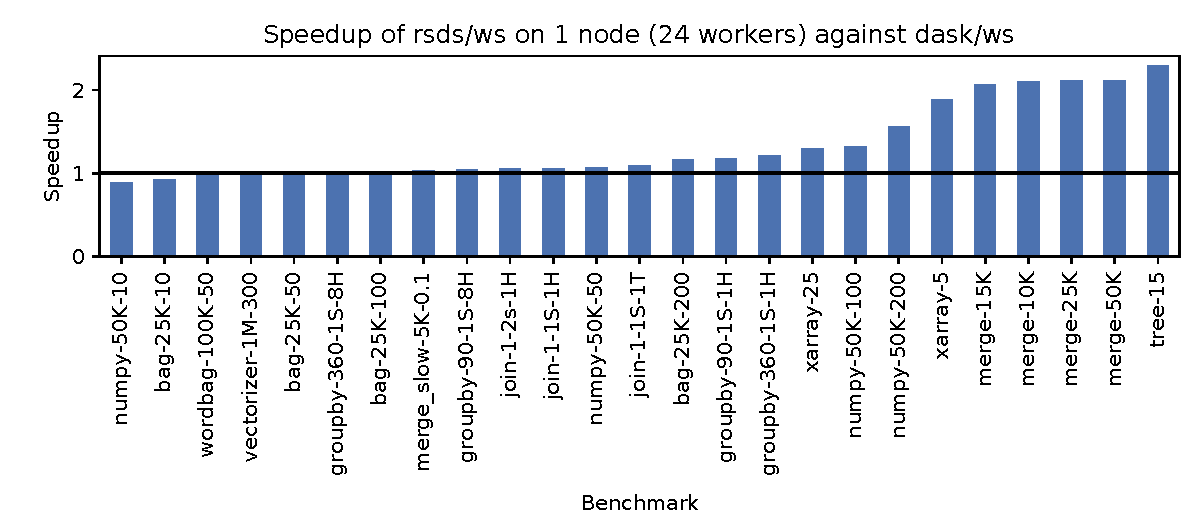
\includegraphics[width=0.8\textwidth]{./imgs/rsds/charts/speedup-rsds-ws-1}
	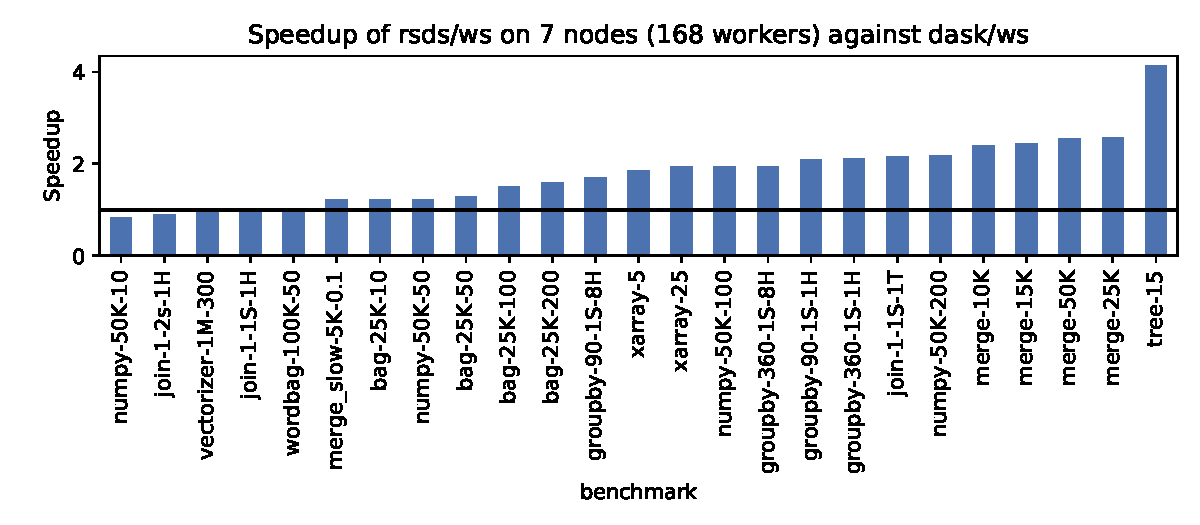
\includegraphics[width=0.8\textwidth]{./imgs/rsds/charts/speedup-rsds-ws-7}
	\caption{Speedup of \rsds{}/ws scheduler; baseline is \dask{}/ws.}
	\label{fig:rsds-dask-ws-all}
\end{figure}

In the first experiment, we have compared the efficiency of the \rsds{} and
\dask{} server implementations on a diverse set of benchmarks, using both the
work-stealing and the random scheduler. The results for the work-stealing schedulers are shown in
\Autoref{fig:rsds-dask-ws-all}. The data confirms our expectation that reducing the overhead of the
server can help improve the makespan of executed task graphs by a non-trivial amount. Even though
\rsds{} uses a much simpler work-stealing scheduler, its more efficient runtime
provides in most cases better performance. This effect is accentuated for a larger cluster with
more workers.

\begin{figure}
	\centering
	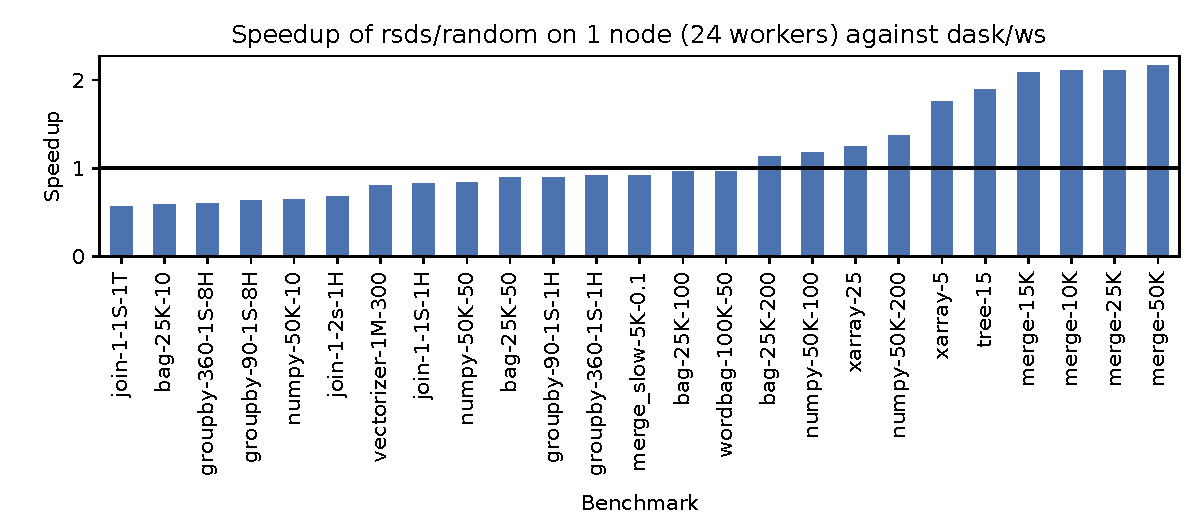
\includegraphics[width=0.8\textwidth]{./imgs/rsds/charts/speedup-rsds-random-1}
	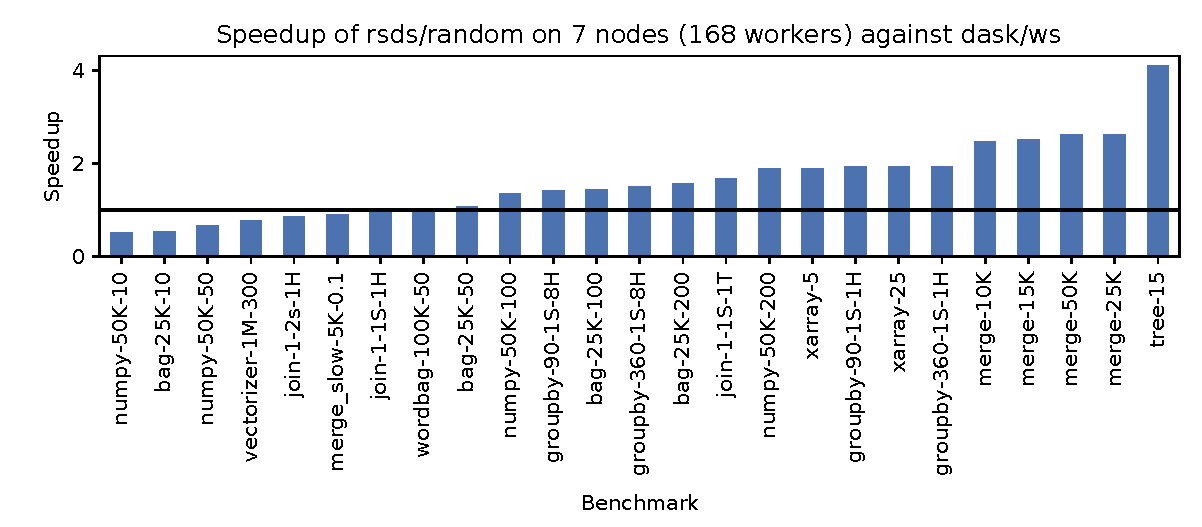
\includegraphics[width=0.8\textwidth]{./imgs/rsds/charts/speedup-rsds-random-7}
	\caption{Speedup of \rsds{}/random scheduler; baseline is \dask{}/ws.}
	\label{fig:rsds-dask-random-all}
\end{figure}

Since the work-stealing implementations of \rsds{} and
\dask{} are not exactly identical, the result above could also be explained by
a difference in scheduling, rather than reduced runtime overhead. To eliminate that possibility, we
have also performed an experiment where we compare \rsds{} using a random
scheduler with \dask{} using its sophihisticated work-stealing scheduler. The
results of this experiment can be seen in \Autoref{fig:rsds-dask-random-all}. They clearly confirm that
the speedup is not caused by \rsds{} having a better scheduler, because even
with a completely random schedule, it is still able to outperform \dask{}. This
serves as an evidence that the improved performance of \rsds{} with
work-stealing is caused by better runtime efficiency, and not by better schedules.

The results of this experiment are summarized in Table~\ref{tab:rsds-geom-mean-speedup}, which shows the
geometrical mean of speedup of the tested \rsds{} configurations, over a
baseline using the \dask{} server with the work-stealing scheduler. The table
also contains the results of the \dask{} server with a random scheduler, to
provide a more complete picture. Even with the random scheduler, \rsds{} is on
average faster than \dask{} using work-stealing. With more workers, this effect
is further increased.

\setlength{\tabcolsep}{5pt}
\begin{table}
	\caption{Geometric mean of speedup over the \dask{}/ws baseline}
	\centering
	\label{tab:rsds-geom-mean-speedup}
	\begin{tabular}{c|c|r|r|r}
		\textbf{Server} & \textbf{Scheduler} & \textbf{Node count} & \textbf{Worker	count} &
		\textbf{Speedup}                                                                                 \\
		\midrule
		dask            & random             & 1                   & 24                   & $0.88\times$ \\
		rsds            & random             & 1                   & 24                   & $1.04\times$ \\
		rsds            & ws                 & 1                   & 24                   & $1.28\times$ \\
		dask            & random             & 7                   & 168                  & $0.95\times$ \\
		rsds            & random             & 7                   & 168                  & $1.41\times$ \\
		rsds            & ws                 & 7                   & 168                  & $1.66\times$ \\
	\end{tabular}
\end{table}

In~\Autoref{sec:rsds-dask-overhead-analysis}, it was noted that the random scheduler used in
\dask{} was quite competitive with the work-stealing scheduler implementation.
Our hypothesis was that this phenomenon is reinforced by the runtime overhead of
\dask{}. To test this hypothesis, we have also compared the performance of the
random scheduler in \rsds{} vs its work-stealing implementation. The results
can be observed in \Autoref{fig:rsds-random-baseline}. We can see that in the case of
\rsds{}, the random scheduler is less competitive (you can compare the results
with \Autoref{fig:dask-ws-vs-random}), and does not significantly outperform work-stealing in any of
the benchmarked cases. This suggests that with a more reasonable runtime overhead of the server, a
work-stealing scheduler is strictly better than a random scheduler, which is a much more intuitive
result.

\begin{figure}
	\centering
	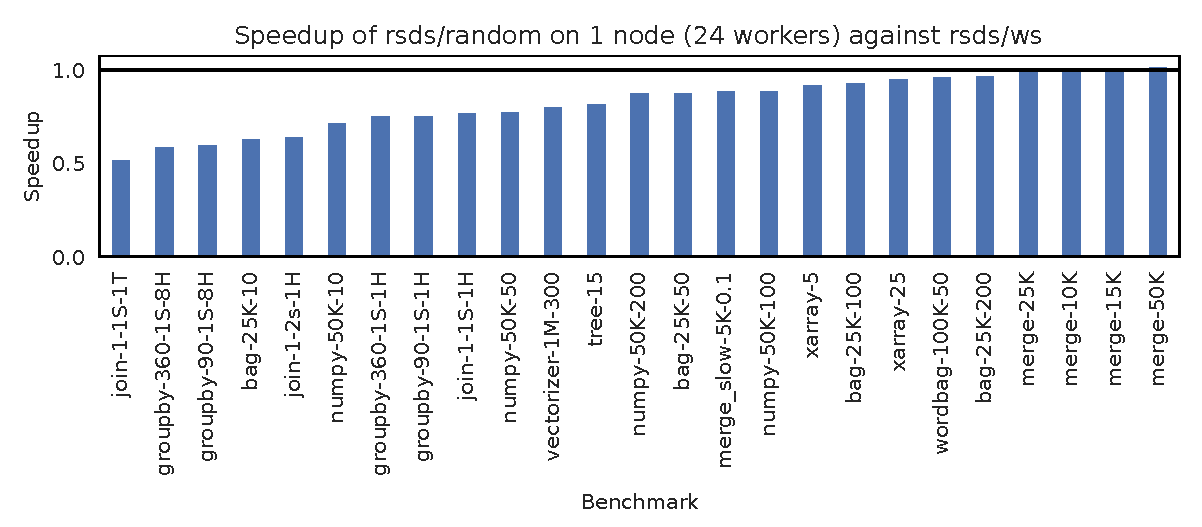
\includegraphics[width=0.9\textwidth]{./imgs/rsds/charts/speedup-rsds-random-1-baseline-rsds-ws}
	\caption{Speedup of \rsds{}/random scheduler; baseline is \rsds{}/ws.}
	\label{fig:rsds-random-baseline}
\end{figure}

To provide a clearer comparison of these results, Table~\ref{tab:rsds-random-geom-mean-speedup} shows the
geometric mean of speedup of the random scheduler, compared to a work-stealing scheduler baseline
of a corresponding server implementation. It is clear from the results that in
\rsds{}, the random scheduler is less performant (relative to its work-stealing
counterpart), than in \dask{}.

\setlength{\tabcolsep}{5pt}
\begin{table}
	\caption{Geometric mean of speedup for random schedulers}
	\centering
	\label{tab:rsds-random-geom-mean-speedup}
	\begin{tabular}{c|c|r|r|r|r}
		\textbf{Server}      & \textbf{Scheduler} & \textbf{Baseline} & \textbf{Node count} &
		\textbf{Worker	count} & \textbf{Speedup}                                                   \\
		\midrule
		dask                 & random             & dask/ws           & 1                   & 24
		                     & $0.88\times$                                                       \\
		rsds                 & random             & rsds/ws           & 1                   & 24
		                     & $0.82\times$                                                       \\
		dask                 & random             & dask/ws           & 7                   & 168
		                     & $0.95\times$                                                       \\
		rsds                 & random             & rsds/ws           & 7                   & 168
		                     & $0.85\times$                                                       \\
	\end{tabular}
\end{table}

\subsection*{Scaling comparison}
One of the motivations for implementing \rsds{} was to improve the performance
of \dask{} workflows in \gls{hpc} scenarios. In these
use-cases, it is important for the runtime to scale to a large amount of workers, which can be
provided by an \gls{hpc} cluster. We have designed an experiment which tests the
strong scaling of both server implementations on several cluster sizes, ranging from
$1$ node ($24$ workers) to $63$
nodes ($1512$ workers). The default, work-stealing scheduler was used for both
server implementations.

\begin{figure}[h]
	\centering
	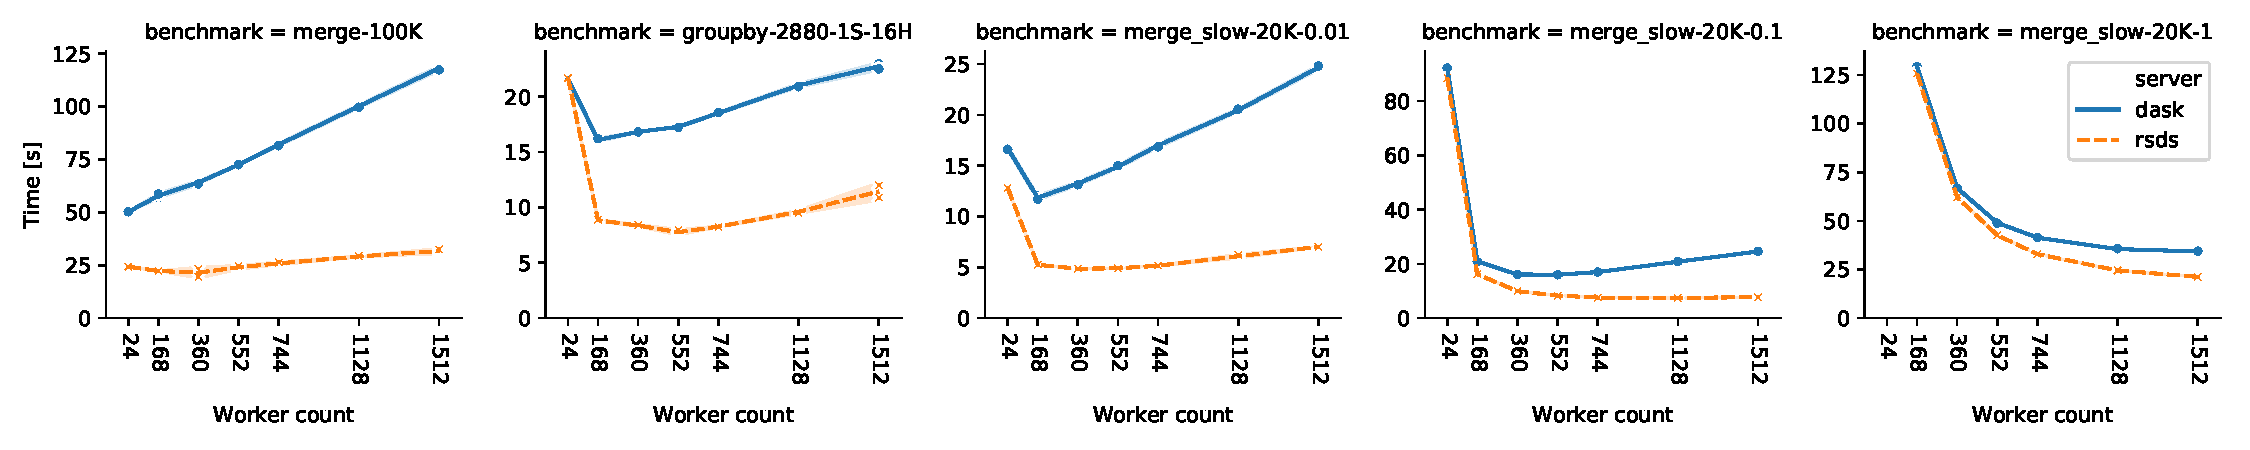
\includegraphics[width=0.8\textwidth]{./imgs/rsds/charts/rsds-dask-scaling}
	\caption{Strong scaling of \rsds{} vs \dask{} on selected task graphs}
	\label{fig:rsds-dask-scaling}
\end{figure}

The results of this experiment are shown in \Autoref{fig:rsds-dask-scaling}. The first examined task
graph is \texttt{merge-100K}, which executes hundred thousand trivial, almost instant
tasks. It is an adversarial case for a scheduler, as the tasks are short and thus the overhead of
scheduling and network transfers will overcome most parallelism gains. Therefore, increasing the
amount of workers will probably not provide a large speedup for this task graph. However, it should
ideally not slow down the computation to a large extent. We can see that
\rsds{} scales up to $15$ nodes
($360$ workers). This is caused by the fact that the cost associated with
worker management and work-stealing increases with an increasing number of workers, and from some
point it starts to dominate, because the tasks are too short. However, \dask{}
fares much worse. It is twice slower when compared to \rsds{} with a single
worker node, but four times slower with $63$ nodes
($1512$ workers). Here we can see that the inner overhead of
\dask{} adds up, and its performance is reduced significantly with each
additional worker node. On the other hand, with \rsds{}, the total makespan
stays relatively constant, even after it stops scaling.

The next tested benchmark was \texttt{groupby-2880-1S-16H}, which computes an analysis of table data
using a task graph automatically generated by \dask{}, using the
\texttt{DataFrame} \gls{api} inspired by the \texttt{pandas}
interface. This task graph provides many opportunities for parallelization, as the individual tasks
work on a subset of rows and thus have more computational density compared to the
\texttt{merge} task graph. However, Table~\ref{tab:dask-graph-properties} shows that the
average computation time is still only around $10ms$, while the average task
output is $1 MiB$. This benchmark thus produces considerable network traffic.
While both \dask{} and \rsds{} have identical performance
with a single worker node, \dask{} stops scaling at $7$
nodes and further its performance degrades and eventually becomes slower than the single node case.
\rsds{} scales up to $23$ worker nodes, hence it is able
to utilize three times more workers. With more worker nodes, the performance of
\rsds{} also degrades, as the network communication caused by task output
transfers and work-stealing messages starts to dominate the overall execution time. In this case,
\dask{} and \rsds{} follow a very similar scaling pattern,
however, in absolute terms, the makespans are twice shorter with \rsds{}.

The third examined task graph is \texttt{merge\_slow-20K}, which executes twenty thousand tasks,
where each task has a fixed duration, specified by a parameter (note that the
\texttt{merge} and \texttt{merge\_slow} benchmarks have the exact same task
graph shape, the only difference is the duration of each task). We have benchmarked three variants
of this task graph, with $0.01$, $0.1$ and
$1$ second tasks, same as for the previous similar experiment that we have
performed with \dask{} only. This gives us a better idea of the task
granularity required for \dask{} and \rsds{} to scale
effectively. With $10$ millisecond tasks, \dask{} scales
to $7$ workers and then its performance follows a similar shape as for
\texttt{merge-100K}. \rsds{} stops scaling at
$15$ nodes, then its performance drops slightly with more added nodes. With
$100$ millisecond tasks, \rsds{} is able to scale up to
$47$ worker nodes ($1128$ workers), from that point on
its performance stagnates. \dask{} scales only up to $23$
worker nodes, then the makespan again starts to increase when additional workers are added. For the
last task graph, with one second tasks, both \rsds{} and
\dask{} scale up to $63$ nodes
($1512$ workers). However, \rsds{} is consistently faster
on all cluster sizes, and its performance in respect to \dask{} increases with
added worker nodes; it is $1.03\times$ faster than \dask{} with
$7$ nodes and $1.6\times$ faster with
$63$ nodes.

In general, \rsds{} is able to scale to a larger number of workers than
\dask{}, thanks to its reduced runtime overhead. Furthermore, it is also able
to keep its performance relatively steady with an increasing number of workers, even after it stops
scaling, even for short tasks.

\subsubsection*{Overhead per task}
In~\Autoref{sec:dask-overhead-per-task}, we have seen that the average overhead of
\dask{} for each task is around $0.3ms$. In this experiment,
we have measured the per-task overhead of \rsds{}, so that we could qualify how
much was its overhead reduced, relative to the baseline. All the benchmarks in this experiment were
performed with the \emph{zero worker} implementation.

\begin{figure}
	\centering
	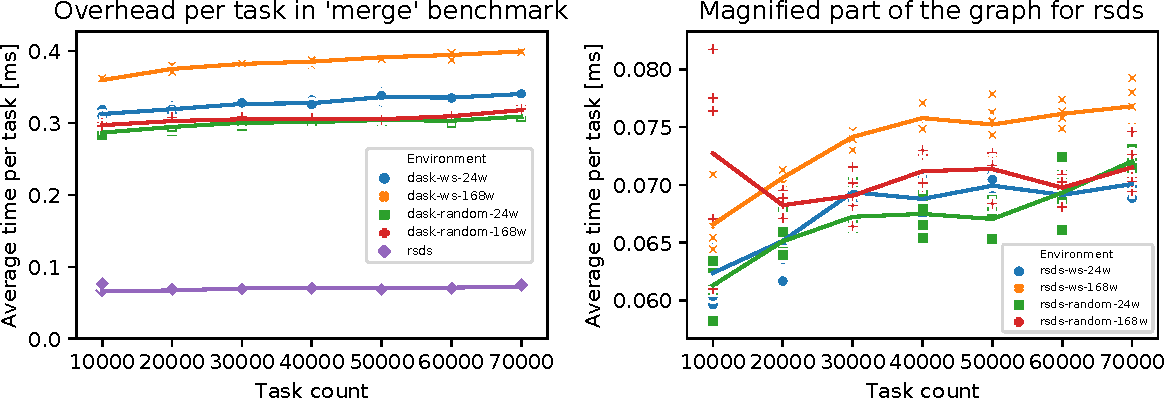
\includegraphics[width=0.8\textwidth]{./imgs/rsds/charts/rsds-merge-task-scaling}
	\caption{Overhead per task for \rsds{} and \dask{} with an
	increasing number of tasks.}
	\label{fig:rsds-merge-task-scaling}
\end{figure}

We have performed the same experiment as with \dask{}, to calculate the
per-task overhead on the \emph{merge} benchmark. \Autoref{fig:rsds-merge-task-scaling} shows
how does the per-task overhead change for larger task graphs. From the chart on the left side, we
can see that the per-task overhead of \rsds{} is approximately
$3-4$ times smaller than the overhead of \dask{}. From
this chart, it looks like its overhead stays constant with an increasing number of tasks, yet when
we zoom in on the section containing \rsds{} results (which we can see in the
chart on the right side), we can observe a similar pattern that we see for
\dask{} -- the overhead of the work-stealing scheduler increases slightly with
more tasks, and the work-stealing scheduler has a larger overhead than the random scheduler, in
general. However, it happens on a much smaller absolute scale than with
\dask{}.

\begin{figure}
	\centering
	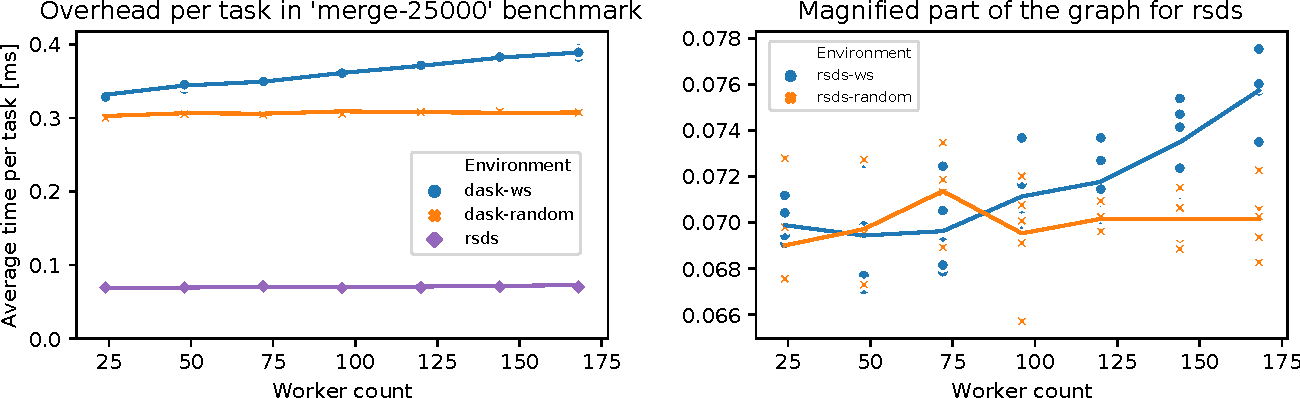
\includegraphics[width=0.8\textwidth]{./imgs/rsds/charts/rsds-merge-worker-scaling}
	\caption{Overhead per task for \rsds{} and \dask{} with an
	increasing number of workers.}
	\label{fig:rsds-merge-worker-scaling}
\end{figure}

\Autoref{fig:rsds-merge-worker-scaling} depicts the results of per-task overhead for an increasing
number of workers. The results are almost identical, the overhead of \rsds{} is
several times smaller than with \dask{}, and it increases for the work-stealing
scheduler slightly with more added workers. Athough this increase is so small that it is almost
negligible, at least for the benchmarked number of workers.

\begin{figure}
	\centering
	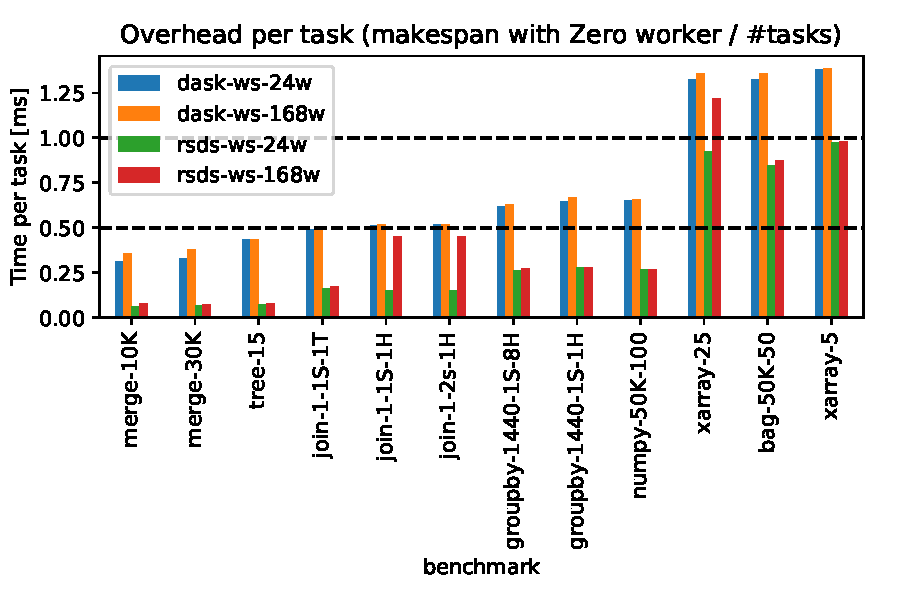
\includegraphics[width=0.8\columnwidth]{./imgs/rsds/charts/rsds-dask-overhead-all}
	\caption{Overhead per task for various cluster sizes and benchmarks}
	\label{fig:rsds-dask-overhead-all}
\end{figure}

In order to confirm that the per-task overhead results from the \emph{merge}
benchmark generalize to other benchmarks, we have also performed a similar experiment for several
other task graphs. The results of this experiment are shown in Figure\ref{fig:rsds-dask-overhead-all}.
We can see that the overhead for the \emph{merge} benchmark is on the lower end of
the spectrum, and it reaches up to $1.25$ ms for some other benchmarks. The
results show that the per-task overhead of \rsds{} is always smaller then the
overhead of \dask{}, however the difference is not that large for the
\emph{xarray} and \emph{bag} benchmarks.

\begin{figure}
	\centering
	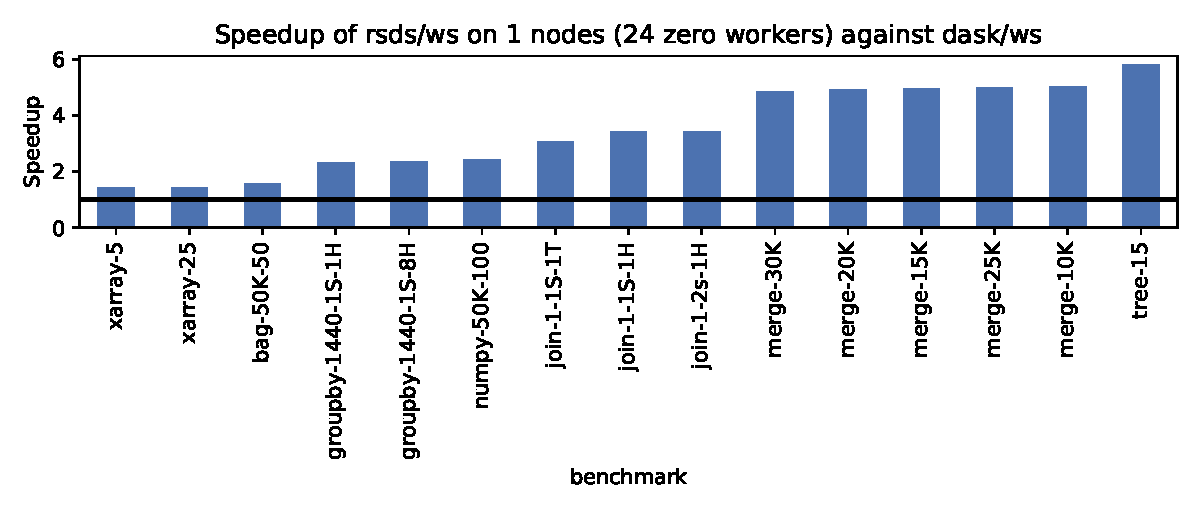
\includegraphics[width=0.9\textwidth]{./imgs/rsds/charts/speedup-zw-rsds-ws-1}
	\caption{Speedup of \rsds{}/ws over \dask{}/ws with the zero worker
	implementation}
	\label{fig:rsds-zero-worker-speedup}
\end{figure}

To evaluate the end-to-end effect of overhead on task graph makespan, we have executed several
benchmarks with the \emph{zero worker} implementation, and compared their overall
makespan, for both \dask{} and \rsds{}. Note that we could
not have evaluated all the benchmarks with the zero worker, since some of the benchmark task graphs
depend on the actual computed contents of data objects generated by tasks, however the zero worker
implementation does not execute tasks, and it is thus not able to generate the correct data. The
results of this benchmark can be found in \Autoref{fig:rsds-zero-worker-speedup}. In all the tested
benchmarks, \rsds{} produced shorter makespans than
\dask{}; in some cases it was up to six times faster. This speedup is larger
than with the standard worker implementation; this shows that if the overhead of the worker was
further reduced, \rsds{} could futher improve its performance advantage over
\dask{}. In other words, \rsds{} would benefit more from a
faster worker implementation than the \dask{} server could.

All these experiments have shown that \rsds{} exhibits similar performance
behavior and scaling patterns as \dask{}, which is not surprising, given that
it reuses its client and worker implementations. However, the most important result is that in
absolute terms, it tends to be faster than \dask{}, across various task graphs
and cluster sizes. The overall overhead present in the whole \rsds{} cluster
could be further reduced e.g.\ by also implementing the worker (or even the client) in another
language than Python, however that would probably make it quite challenging to keep backwards
compatibility with existing \dask{} programs.

\section{Summary}
We have analysed the performance of the \dask{} task runtime on a set of
diverse benchmarks in an \gls{hpc} setting. Our analysis has demonstrated that
\dask{} is heavily bottlenecked by the runtime overhead of its Python
implementation, and also by other aspects related to the usage of Python, notably the presence of
the \gls{gil}. This suggests that further optimisations should focus mainly on
the overhead of its server, rather than its scheduler, as even a completely random scheduler is
able to achieve quite reasonable performance, since the schedule is not the primary bottleneck, at
least in certain cases.

To improve the performance of \dask{} workflows, we have developed
\rsds{}, an open-source drop-in replacement for the \dask{}
server\footnoteurl{https://github.com/it4innovations/rsds}. It was built from the ground up with a focus on runtime
efficiency and scheduler modularity, but at the same time we have designed it to be compatible with
the original \dask{} protocol, which means that it is backwards-compatible with
existing \dask{} programs, and can be used to speed them up.

We have performed a series of experiments where we have compared the performance of
\rsds{} vs \dask{}. The results of our experiments indicate
that optimizing the runtime is definitely a worthy effort to pursuit, as
\rsds{} has been able to outperform \dask{} in various
scenarios, even though it uses a much simpler work-stealing scheduling algorithm.

After we had an indication that \rsds{} can be used to improve the efficiency
of existing \dask{} workflows, we have contacted the authors and maintainers of
\dask{}, and discussed the \rsds{} approach with
them\footnoteurl{https://github.com/dask/distributed/issues/3139}\footnoteurl{https://github.com/dask/distributed/issues/3783}\footnoteurl{https://github.com/dask/distributed/issues/3872}. Some of its
ideas have been since adapted in the \dask{} project and led to improving its
performance.
